\documentclass{chi2009}

\usepackage{ifthen, times, url, graphics, color, epstopdf}

\usepackage[pdftex]{hyperref} 

\hypersetup{
pdftitle={Designing Incentives for Inexpert Human Raters},
pdfauthor={Aaron Shaw, John Horton, Daniel Chen},
pdfkeywords={Search, Amazon Mechanical Turk, Human Computation,
  Crowdsourcing, Experimentation},
bookmarksnumbered,
pdfstartview={FitH},
colorlinks,
citecolor=black,
filecolor=black,
linkcolor=black,
urlcolor=black,
breaklinks=true,
}
\newcommand{\comment}[1]{}
\definecolor{Orange}{rgb}{1,0.5,0}
\newcommand{\todo}[1]{\textsf{\textbf{\textcolor{Orange}{[[#1]]}}}}

%\pagenumbering{arabic}  % Arabic page numbers for submission.  Remove this line to eliminate page numbers for the camera ready copy

\usepackage{threeparttable, longtable, booktabs}

\begin{document}
% to make various LaTeX processors do the right thing with page size
\special{papersize=8.5in,11in}
\setlength{\paperheight}{11in}
\setlength{\paperwidth}{8.5in}
\setlength{\pdfpageheight}{\paperheight}
\setlength{\pdfpagewidth}{\paperwidth}

% use this command to override the default ACM copyright statement 
% (e.g. for preprints). Remove for camera ready copy.
\toappear{Permissions to come.}

\title{Designing Incentives for Inexpert Human Raters} 

\numberofauthors{3}

%\author{
%\alignauthor Anonymous
%}

%\begin{comment} 
\author{
\alignauthor 
Aaron D. Shaw\\
       \affaddr{UC Berkeley}\\
       \affaddr{410 Barrows Hall \#1980}\\
       \affaddr{Berkeley, CA 94720}\\
       \affaddr{adshaw@berkeley.edu}
\alignauthor 
John J. Horton\\
       \affaddr{Harvard University}\\
       \affaddr{383 Pforzheimer MC}\\
       \affaddr{56 Linnaean St}\\
       \affaddr{Cambridge, MA 02138}\\
       \affaddr{horton@fas.harvard.edu}
\alignauthor 
Daniel L. Chen\\
       \affaddr{Duke University}\\
       \affaddr{Science Dr \& Towerview Rd}\\
       \affaddr{Office 3020}\\
       \affaddr{Durham, NC 27708}\\
       \affaddr{dchen@law.duke.edu}
}
%\end{comment} 

\maketitle

\begin{abstract} 
The emergence of online labor markets make it far easier to use
individual human raters to evaluate materials for data collection and
analysis in the social sciences. In this paper, we report the results
of an experiment---conducted in an online labor market---that measured
the effectiveness of a collection of social and financial incentive
schemes for motivating workers to conduct a qualitative, content
analysis task. Overall, workers performed better than chance, but
results varied considerably depending on task difficulty. We find that
treatment conditions which asked workers to prospectively think about
the responses of their peers---when combined with financial
incentives---produced more accurate task performance. Other
treatments generally had weak effects on quality. Non-US workers
performed significantly worse than US workers, regardless of treatment
group.
\end{abstract}

% A category with the (minimum) three required fields
\category{H.5.2}{Information Interfaces and Presentation}{Interaction Styles}
\category{H.3.3}{Information Storage and Retrieval}{Information Search and Retrieval}
\category{J.4}{Social and Behavioral Sciences}{Economics, Sociology}

\terms{Economics, Sociology, Experimentation, Human Factors, Measurement}
\keywords{Search, Amazon Mechanical Turk, Human Computation,
  Crowdsourcing, Experimentation, Content Analysis}

\section{Introduction}
The binding constraint in much observational, empirical social
science research is finding data with useful, well-measured indepedent
and dependent variables. Often, compelling research questions require the quantification of complex constructs such as trustworthiness, beauty, or aggression. Since these kinds of measures are unlikely to appear in observational data sets, researchers must look at primary source material and then classify it according to some scheme. A recent economic
  example used the photograph-based characterizations trustworthiness
  of people asking for loans on the social lending site
  \href{http://www.prosper.com}{Prosper.com} and then used these
  ratings to predict their outcomes\cite{duarte2009tc. Another
  example used inexpert, amateur evaluations of short debate clips
  from gubernatorial elections and found that these evaluations were
  predictive\cite{benjamin2009}. Often times these qualitative coding tasks require human judgment, but do not require any expertise. This makes them ripe for delegation to inexpert raters, yet the tasks are often tedious and time-consuming, and finding research assistance to perform the tasks is difficult or expensive. 
% cut from line 107 above:
% For economists, the problem is less acute
%since many of the independent variables, such as income, education
%levels, etc., are measured reliably with little error.  However, even
%in economics, more papers are being written that try to quantify and
%then use more fluid concepts or attributes like trustworthiness,
%reputation, beauty or aggression to predict social phenomena.

An emerging phenomenon---the online labor market---can scale the process of qualitative coding (also known in some social science circles as ``content analysis'') using large numbers of non-experts. However, it remains difficult to elicit and synthesize high-quality judgments from non-expert raters collaborating remotely through online labor markets. Among the foremost practical challenges of this kind, the design of optimal incentives schemes to facilitate this peculiar form of cooperative work has received scant scholarly attention. Prior economic, sociological, and psychological research offers much theoretical guidance, but little empirical evidence as to the sorts of incentives that elicit the highest quality judgments from non-expert raters. 

In this paper, we present the results of a controlled experiment that directly compares the effects of fourteen different incentive schemes within the context of an online labor market. The incentive schemes encompass a wide variety of existing research into human cooperation, labor, motivation, and behavior. We test the incentives using a single non-expert content analysis task, for which we obtained validated answers prior to administering the experiment. We then compare the aggregate performance of workers in the different treatment conditions in order to determine which incentive schemes elicit the most accurate judgments in comparison to the control condition. 

\subsection{Use of Online Labor Markets}
In online labor markets, workers from around the world perform data
processing tasks for money. While some sites focus on skilled work
like computer programming (e.g., oDesk, Elance, Guru), Amazon's
\href{https://www.mturk.com/mturk/welcome}{Mechanical Turk} (MTurk) is
intended for small, simple and discrete tasks and thus is probably the
most directly useful for researchers. The challenge of tapping this
resource is that raters are inexpert and there is sometimes a high
degree of inter-rater disagreement, regardless of the measure.  The
low cost of raters make large numbers of ratings possible, but this
volume of data also prohibits a hand-curated approach to selecting
high-quality raters.\footnote{Several innovative start-up companies,
  such as Crowdflower are offering services as intermediaries. Clients
  bring them tasks amenable to the crowdsourcing approach and they
  break the tasks down, recruit workers and ensure quality results.}

Several papers in the computer science literature have used online
labor markets such as MTurk to conduct experiments
\cite{kittur2008crowdsourcing, snow2008cheap, sheng2008get}. Horton,
Rand, and Zeckhauser discuss the social science potential of online
experiments in these markets, focusing on how challenges to validity
can be overcome \cite{hortonZeck2010}. There already exists a small
literature on crowdsourcing from a social science perspective
\cite{huberman-crowdsourcing, mason2009fip, horton2010labor,
  chen2009}. New tools are also being developed that make
experimentation easier \cite{little-turkit}.

\subsection{Obtaining Quality Work} 
% TK-JH maybe worth clarifying intensive/extensive margin jargon for non-economists?
In online labor markets, the usual rules of labor supply generally
apply: pay more money and you can attract more workers on both the
extensive margin (i.e., more workers are willing to participate at all) and the 
intensive margin (i.e., workers that participate work longer or produce more). However, attracting more workers does
not necessarily lead to better work. 

Earlier work \cite{von2004labeling, ipeirotis2010, snow2008cheap,
  Hopkins-King2010, downs2010your} has focused on techniques for filtering and
processing judgments of inexpert human raters. By contrast, we focus
on how to produce better judgments in the first place.

Some work has already been done in this vein. A recent experimental
paper by Chandler and Kapelner \cite{chandler2010}, conducted in
MTurk, looked at how knowledge about the purpose of a task affected
quality and labor supply. US-based subjects that knew they were
labeling cancer cells in an image produced more output than those not
similarly informed.  Interestingly, they found no evidence of similar
effects for non-US workers. The same authors also recently conducted
an experiment in which they demonstrated that slowing down the presentation of 
survey questions increased comprehension \cite{kapelnerpreventing}. 
% TK-JH - not sure what these were for...I inserted some into the paragaph above
%\cite{von2004labeling}
%\cite{huberman-crowdsourcing}
%\cite{law2003tagatune}
%\cite{ipeirotis2010,hortonZeck2010}.
%\cite{mason2009fip}
%\cite{horton2010labor}
\subsection{Content Analysis}
In some kinds of research, human judgments can be evaluated against
objective, correct answers. This is the case for tasks such as image
labeling or character recognition, where accurate automated techniques
remain costly or unavailable. In others, human judgments are important
precisely because they incorporate subjective perceptions, which may
be central to the topic of study. This is the case for many types of
content analysis tasks, where researchers aim to identify certain
qualities or patterns in textual materials that evade automated
detection. In both objective and subjective variants, the challenge of
developing techniques to aggregate individual judgments as well as to
assess their precision and accuracy has given rise to several
different methodological techniques, some of which we review as
background to the method we used in this study.

Useful methodological approaches to this type of problem have emerged
among scholars conducting content analysis of textual materials. Until
recently, content analysis techniques have relied on multiple
researchers implementing a qualitative labeling or coding scheme of
the same text(s), and then using specifically adapted correlation
statistics to evaluate inter-rater (or intercoder) reliability
\cite{krippendorff_content_2003, cohen_coefficient_1960}. The primary
advantage of these approaches lies in the ability to measure
empirically the reliability of seemingly subjective observations. The
cost of such precision, however, is often quite high in terms of time
and labor, making such analysis prohibitively expensive when the scale
of data collection and analysis grows large. Recent work by Hopkins
and King have demonstrated how machine-learning tools and techniques
can be applied to overcome these limitations while retaining high
confidence in the precision and accuracy of results
\cite{Hopkins-King2010}.

\subsection{Our Approach} 
A variety of papers across the social science disciplines have studied
human motivation. This literature is far too voluminous to summarize
here; much of it is also captured by folk wisdom or even in management
cliches. What is certainly not known is the relative merits of
different motivations and how they apply in online contexts. For
example, does offering workers more money improve effort and hence
quality? This lack of knowledge motivated this study, in which we
created a large number of treatment groups and recruited a vast number
of subjects. While this ``kitchen sink'' approach creates some
problems of analysis, we do get breadth even at the expense of
depth. We review the different motivational frameworks in greater
depth below.

\subsection{Our Task} 
%task overview
For our task, we asked subjects to complete a set of six closed-ended,
qualitative content analysis questions using an online survey
interface. All workers in all treatment groups (except one of the two
control groups, which only answered demographic questions) were
directed to analyze the \href{http://www.kiva.org}{Kiva.org} website and then presented with the same
six questions in the same order and with the same answer choices
through the survey interface. The questions asked subjects to conduct
content analysis similar to that used in an earlier study by
\cite{benklershaw2010} to assess U.S. political blogs. For any
questions, workers could choose to leave a blank response.


\subsection{Overview of Results} 
How did the workers recruited from Mechaical Turk (``Turkers'') 
perform on the five content analysis tasks that we
asked them to complete? The results varied by question as well as by
treatment condition. On the two easiest questions, the Turkers
uniformly performed much better than random guessing and only a couple
of the treatments seemed to produce any (small) effect at all. By
contrast, the results for the three difficult questions varied more
widely. In one case, the Turkers' performance was much worse than
chance. At the same time, the variance in responses to these questions
also revealed stronger treatment effects. Aggregating the results from
each condition across all five questions, the Turkers performed better
than chance. More importantly, a few treatments emerged as the clear
winners of our horse race, producing significant improvements in
average answer quality when compared against the control condition. We
discuss the experimental design, data collection, and results in
greater depth below.

\section{Methods and Materials}

\subsection{Content Analysis Task}

%gold standard data
In order to establish a reliable standard against which to judge the
performance of the workers, we also administered the same questions
about the same website through an identical web interface to a group
of five research assistants prior to conducting the experiment. On all
of the questions included in the study, at least four of the five
research assistants gave identical responses, suggesting a high degree
of intercoder reliability. Independent of the research assistants,
Shaw also collected his own answers to the questions, agreeing
with the prevailing answer provided by the research assistants in
every case. We used these responses as validated (i.e., gold standard)
answers to each question.

%detailed description of evaluation task questions
% TK-AS insert link or image of actual task interface
The first two questions followed a multiple choice format, in which
subjects were asked to identify whether (1) a privacy policy; and (2)
``avatars'' or other visual representations of user identities were
present on the site. For both of these questions an ``uncertain''
answer choice was also available. The third and fourth questions asked
subjects to assess how frequently members of the site engaged in
specific behaviors (ranking or rating (3) content and (4) other users)
using a five point scale ranging from ``Very frequently'' to ``Very
rarely or never.''  Finally, the last two questions asked subjects to
identify whether specific features related to (5) social networking
and (6) revenue creation were present or not on the site. In these
last two, subjects could check boxes to select any combination of
answer choices from a pre-defined list.

The first of the six questions (about whether or not the site had a
privacy policy) was presented prior to treatment. We report the
results for this pre-treatment question but do not include it as part
of our outcome performance measurement.  A copy of the questions as they appeared in the experimental interface is
available on Horton's website.\footnote{\href{\http://goo.gl/9CVa5}{http://goo.gl/9CVa5}
}


%dependent variable: evaluation task performance
The dependent variable of our study was the number of correct answers
to the five post-treatment information seeking questions per
worker.\footnote{In the case of the checkbox questions -- numbers (5)
  and (6) -- we coded any response including the gold standard answer
  as correct. Obviously, in the case of a question where we did not
  know the correct answer ahead of time, a much different process
  would be needed to identify the best response. As such filtering
  processes were not the focus of this study, we refer consideration
  of this topic to the work of others.\cite{snow2008cheap}} We
considered blank responses incorrect answers for all questions. After
coding responses to identify which ones each worker answered correctly
(i.e., in agreement with the gold standard response), we aggregated
the number of correct answers per worker. The outcome measure is
therefore an integer (count) with a value between zero and five. As we
describe in further detail below, the workers on MTurk performed
better than chance - estimated as random guessing between all
available answer choices for every question - on four of the five
post-treatment questions.

%demographic control questions
The demographic questions asked workers to provide their age; gender;
country of residence; education level; language skills; employment
status; household size; and internet skills. We included them to
increase precision in our treatment estimates as well as to verify
that our randomization was valid (we discuss the rationale for this
choice in further detail below).
%TK-AS (insert citation to relevant sources for questions)

\subsection{Conduct of the experiment}

%recruitment
Recruitment was conducted through the MTurk online labor market, where
we advertised a brief information seeking task. Recruitment materials
included a description of the study as well as a set of example
questions, all of which were included in the actual job, but none of
which were among the post-treatment questions included in our outcome
variables of interest. Subjects were not informed that they were
participating in a study at the time of recruitment so as to preserve
the ``natural'' environment of the field experiment in the online
labor market. In the task description, we explained that workers would
be paid \$0.30 for completing the task. Given the length of the
assignment and the fact that workers could only complete our job once
(many jobs on MTurk allow workers to return multiple times), this
payment rate was comparable with many other jobs posted to the MTurk
marketplace.

%description of treatment assignment, data collection
Upon agreeing to accept the task on the MTurk website, subjects were
instructed to click a hyperlink pointing to a private server at an
anonymized URL. While we were not able to collect data on how many
individuals saw our recruitment materials, once a worker accepted our
task, their unique MTurk user id was simultaneously assigned randomly
to one of the treatment or control conditions and (together with their
IP address and the information about treatment assignment) stored by a
database on our server. As a result, we were able to use these
different pieces of stored identifying information to block individual
subjects from completing the study more than once or from being
exposed to more than one of the experimental manipulations. While
there is some possibility that individuals could possess more than one
account on the MTurk platform and thereby might have circumvented
these protections, such behavior is expressly prohibited by the site's
terms of service and Amazon actively polices violations (indeed, one
of the authors of the study had the somewhat embarassing experience of
losing his MTurk account as a result of attempting to create multiple
user names in order to test a pilot version of an earlier
study). Furthermore, the payoff for circumventing the system
protections on our job (which required a little more than 2000 unique
judgments) were very low in comparison with some of the large scale
jobs on the site that frequently elicit hundreds of thousands or even
millions of individual judgments. As a result, we feel confident in
the integrity of both the randomization as well as the different
treatment conditions.

%narrative of task completion 
Once Turkers clicked through to our server, the experimental
instrument was then administered through a web-based survey
interface. Subjects arriving at the site were presented with the
version of the instrument corresponding to their treatment assignment
on a single page. Each version of the instrument began with some
general instructions about the task, and (in all conditions except for
the demographic control) a link to the URL of the site that would
serve as the topic of the questions
(\href{http://www.kiva.org}{Kiva.org}). These were followed by several
pre-treatment questions about the site. Then, we introduced the
experimental manipulations (usually consisting of a block of text)
followed by the post-treatment questions and any treatment-specific
materials. Finally, the instruments concluded with a series of
demographic questions.

\subsection{Overview of Treatments: Social, Financial, and Hybrid Incentives}

The experimental manipulations we introduced consisted of framing the
information seeking task in distinct ways using a series of ``social''
and ``financial'' incentives. Together, these different incentive
schemes encompass a number of salient theories of human motivation and
range across several social science disciplines. Generally speaking,
the more social incentives emphasized non-monetary rewards or
punishments for performing our information seeking task whereas the
financial incentives offered explicit monetary performance rewards or
punishments. Some frameworks were hybrids that combined social and
financial incentives. In total, we tested fourteen different incentive
frameworks and compared worker performance in each condition against a
control condition that involved no framing incentives beyond the
baseline compensation offered for completing the job. We also included
a second control group in which workers responded only to the
pre-treatment and demographic questions used in the other
conditions. All workers who completed the task were given the baseline
compensation. Because of some technical complications, we ended up
paying all workers the largest amount they could have received from
their experimental treatment, to avoid potentially under-paying
deserving workers.

All control and treatment conditions are described in further detail
below. For each of the treatment conditions (listed in bold) we have
noted in parentheses whether it is social, financial or hybrid in
nature and included the full treatment text. Where appropriate, we
have also included references to relevant studies in which comparable
incentives were found to effect behavioral outcomes.

\subsection{Control Conditions} 
% TK-JH: Was there something you wanted to add about control here?

\begin{description}
\item[Control] Workers were presented with all pre-treatment, post-treatment and demographic questions.
\item[Demographic] Workers were presented with pre-treatment and demographic questions only.\footnote{Whenever possible, the demographic questions were taken verbatim from the 2005 codebook of the World Values Survey \cite{world_vals_survey2009}. As we described later in the paper, we also borrowed two questions about Internet-use skills from Eszter Hargittai \cite{hargittai2009update}.}
\end{description}

\subsection{Treatment Conditions}

\begin{description}
\item[Tournament scoring (social)] ``For some of the following five questions, you will be in competition against another worker. After this HIT is completed, we will compare your accuracy on these questions against the accuracy of another worker who we will select at random. We will report the results of the competition to you when we process your payment.''%[TK-AS citation]

\item[Cheap Talk---Surveillance (social)] ``After this HIT has been
  completed, your answers to these questions will be reviewed for
  accuracy.'' %[TK-AS citation]
\item[Cheap Talk---Normative (social)] ``It is your job to provide
  accurate answers to these question. It is important that you do your
  job well.'' %[TK-AS citation]
\item[Solidarity (hybrid)] ``For some of the following five questions,
  you have been assigned to the Red team. You and your teammates have
  the opportunity to earn bonuses based on your collective
  performance. After the HIT has been completed, we will verify the
  answers that you all submitted for these questions (independent of
  the website you are analyzing) and compare your team's performance
  with another group of workers completing this HIT. If your team
  wins, you will all receive a bonus.'' %[TK-AS citation]
\item[Humanization (social)] ``Before you complete the questions, I
  just wanted to thank you again for doing this work. My name is
  Aaron.''\footnote{This treatment text was accompanied by a photo of one of the authors.} %TK-Anonymized
\item[Trust (social)] ``Thank you for completing the first set of
  questions. Here is your confirmation code, which you may paste into
  the field on the original HIT page at any time to receive
  payment. We trust that you will still complete the questions below
  to the best of your ability. Your confirmation code and payment for
  this HIT will not change based on the answers you
  submit.''\footnote{In order to make this treatment condition consistent with the design of all other conditions, all workers were asked to submit a completion code when they finished the job. In every condition except this one, we provided these completion codes once the task had been finished and the answers to all questions submitted to our server. Compensation was not conditional on submitting the completion code in any of the conditions.} %[TK-AS
                                                                                                                                                                                                                                                                                                                                                                                                                                                                 %citation]
\item[Normative priming questions (social)] ``Before answering the next
  set of questions about the website, we want to ask you a few
  questions about yourself and your attitudes about
  work.''\footnote{This text was followed by a series of questions drawn from the General Social Survey inquiring about subjects' agreement with statements indicating positive attitudes towards responsibilities and hard work. The statements, in order, were ``People who don't work become lazy''; ``Work is a duty toward society''; ``Work should always come first, even if it means less free time''; ``Work is a person's most important activity''; ``I see myself as someone who does a thorough job.''} %[TK-AS citation - GSS/WVS?]
\item[Reward Accuracy (financial)] ``After this HIT has been completed,
  we will verify the correct answers for at least one of the following
  five questions. For each `trap door' question we will increase your
  total pay by 10\% if you answered it correctly. You will not receive
  this bonus if you do not answer the `trap door' question(s)
  correctly.'' %[TK-JH citation]
\item[Reward Agreement (financial)] ``After this HIT has been
  completed, we will review the answers for at least one of the
  following five questions. For each of the questions we review, we
  will reward you for agreeing with the answers provided by the
  majority of other workers who complete this HIT. The reward will be
  a bonus of 10\% for every agreement.'' %[TK-JH citation]
\item[Punishment Accuracy (financial)] ``After this HIT has been
  completed, we will verify the correct answers for at least one of
  the following five questions. For each one of these `trap door'
  questions we will penalize you 10\% of the bonus that you would have
  received if you answered it incorrectly.'' %[TK-JH citation]
\item[Punishment Agreement (financial)] ``After this HIT has been
  completed, we will review the answers for at least one of the
  following five questions. For each of the questions we review, we
  will penalize you if you disagree with the majority of other workers
  who complete this HIT. The penalty will be a deduction of 10\% from
  the total bonus you could have earned if your answer had agreed with
  the majority.'' %[TK-JH citation]
\item[Promise of Future Work (financial)] ``After this HIT has been
  completed, we will review the performance of each worker on the
  following five questions. If you perform better than average, you
  will have the opportunity to work on future jobs with us.'' %[TK-JH citation]
\item[Bayesian Truth Serum or BTS (financial)] ``For the following
  five questions, we will also ask you to predict the responses of
  other workers who complete this task. There is no incentive to
  misreport what you truly believe to be your answers as well as
  others' answers. You will have a higher probability of winning a
  lottery (bonus payment) if you submit answers that are more
  surprisingly common than collectively predicted.''\footnote{The
    design for this treatment comes from \cite{prelec_bts_2004} who
    used a near identical method in an effort to elicit honest
    opinions from their research subjects. After data collection, the
    responses were subsequently weighted based on the aggregate
    predicted distributions of the respondents. For our own purposes,
    we were merely interested in the question of whether presenting
    our task in a similar way would have a meaningful effect on
    qualitative information seeking. The results we present do not
    involve any of the weighting procedures used by Prelec. We refer
    interested readers to the original paper for more detailed
    information about this technique.}
\item[Betting on Results (financial)] ``For the following five
  questions, you will have the opportunity to win bonuses. After
  completing the questions, we will let you bet a portion of your
  payment on the accuracy of your responses.'' %[TK-JH citation]
\end{description} 

\subsection{Data Collection}
The experiment ran from June 2 through September 23, 2009. During that
time, we collected a total of 2159 unique subjects, of whom 2055
completed the study and 104 dropped out after treatment
assignment. Because we used a random treatment assignment function
(instead of stratified random assignment), the distribution of
subjects across conditions was unequal, ranging between 113 and 167
subjects per condition. Applying Pearson's $\chi^{2}$ test to a
contingency table with the counts of attriters and compliers across
all of the treatment and control groups suggests that attrition was
not significantly different from random (p = 0.919).

Following the completion of data collection, we discovered that
database storing our records from the study had stored inaccurate
values for three of the subjects. As a result, we excluded the results
from these three subjects from all subsequent analysis, with the
exception of the calculation of the total number of subjects assigned
to each treatment group used to generate our estimates of treatment
effects (see below).

\subsection{Statistical Analysis} 

In all of our estimates of treatment effects, we correct for the
increased probability of Type 1 errors when conducting multiple
hypothesis tests in an experiment with many treatments by using the
single-step Bonferroni correction to adjust our p-values
\cite{shaffer1995, hsu1996}. This correction has the advantage of
simplicity as well as strong control of the Familywise Error Rate
(FWER) in a context where the comparisons being tested are unordered
\cite{rosenthalrubin1984}.\footnote{We calculate these corrections
  using the
  \href{http://cran.r-project.org/web/packages/multtest/index.html}{``multtest''}
  package in \href{http://www.r-project.org}{R}.}

We used Intention-To-Treat (ITT) estimators to calculate the average
effect of each treatment compared against the control condition. What
this means practically is that subjects that quit after assignment to
a group were still included in calculations as answering
incorrectly. ITT estimators have the advantage of correcting for
potentially confounding effects of attrition and avoiding the bias
introduced into the analysis of many randomized experimental results
by regression estimates \cite{freedman2008logistic,
  freedman2008multtreat}.

%
%TK-AS maybe insert formula for Bonferroni correction?
%TK-AS maybe insert formula for ITT estimators?

\section{Results}

\subsection{Performance on Individual Questions}
Looking at the percentage of correct responses per question across all
conditions (except demographic control), worker performance varied
significantly from chance (random guessing among the available answer
choices) for all five questions (see Table
\ref{table:ind_q_results}).\footnote{We used $\chi^{2}$ tests for
  goodness of fit to calculate these comparisons between the
  distribution of correct responses and predicted probabilities of
  producing correct answers through random guessing for each
  question.} On four of the five, workers performed better than
chance, whereas the question about revenue streams elicited
performance that was significantly worse than chance.

% table 1 - individual questions
\begin{table}[ht]					% set the layout
\begin{center}						% format the layout
\caption{Performance on Individual Questions (All Conditions)} % table title
\vspace{8pt}
\begin{threeparttable}
\begin{tabular}{@{}l r r@{}}
\toprule
& Actual \% Correct & \% Correct \% w/ ``Noise'' \\
\cmidrule(l){2-3}
Avatars & 73.2 & 25\\ 
Content rank/rate & 25.6 & 20\\
User rank/rate & 28.7 & 20\\
Revenue streams & 47.6 & 50\\
Soc. network features & 62.8 & 50\\
\bottomrule
\end{tabular}
  \begin{tablenotes}[para]
  %\begin{flushleft}
     \small{\item $\chi^{2}$ test indicates all differences significant ($p \leq 0.05$)}
     %\item Test 
   %\end{flushleft}
  \end{tablenotes}
\end{threeparttable}
\label{table:ind_q_results}
\end{center}
\end{table}

% Performance on indiv. questions compared across conditions
Comparing the percentage of correct answers across questions and
across experimental conditions reveals fairly consistent performance
from each treatment group despite the substantial variation
across questions (see Figure \ref{fig:per_q}).\footnote{We did not
  conduct hypothesis tests comparing average treatment effects for
  each question. Such question-level effects were not our primary
  outcome variables in part because of the specificity of the content
  of each question and the fact that we looked at responses only from
  a single website. See the Discussion section below for additional
  consideration of this topic.}

\begin{figure} 
\centering 
\caption{Worker Performance Distribution - All Conditions \label{fig:per_q}}
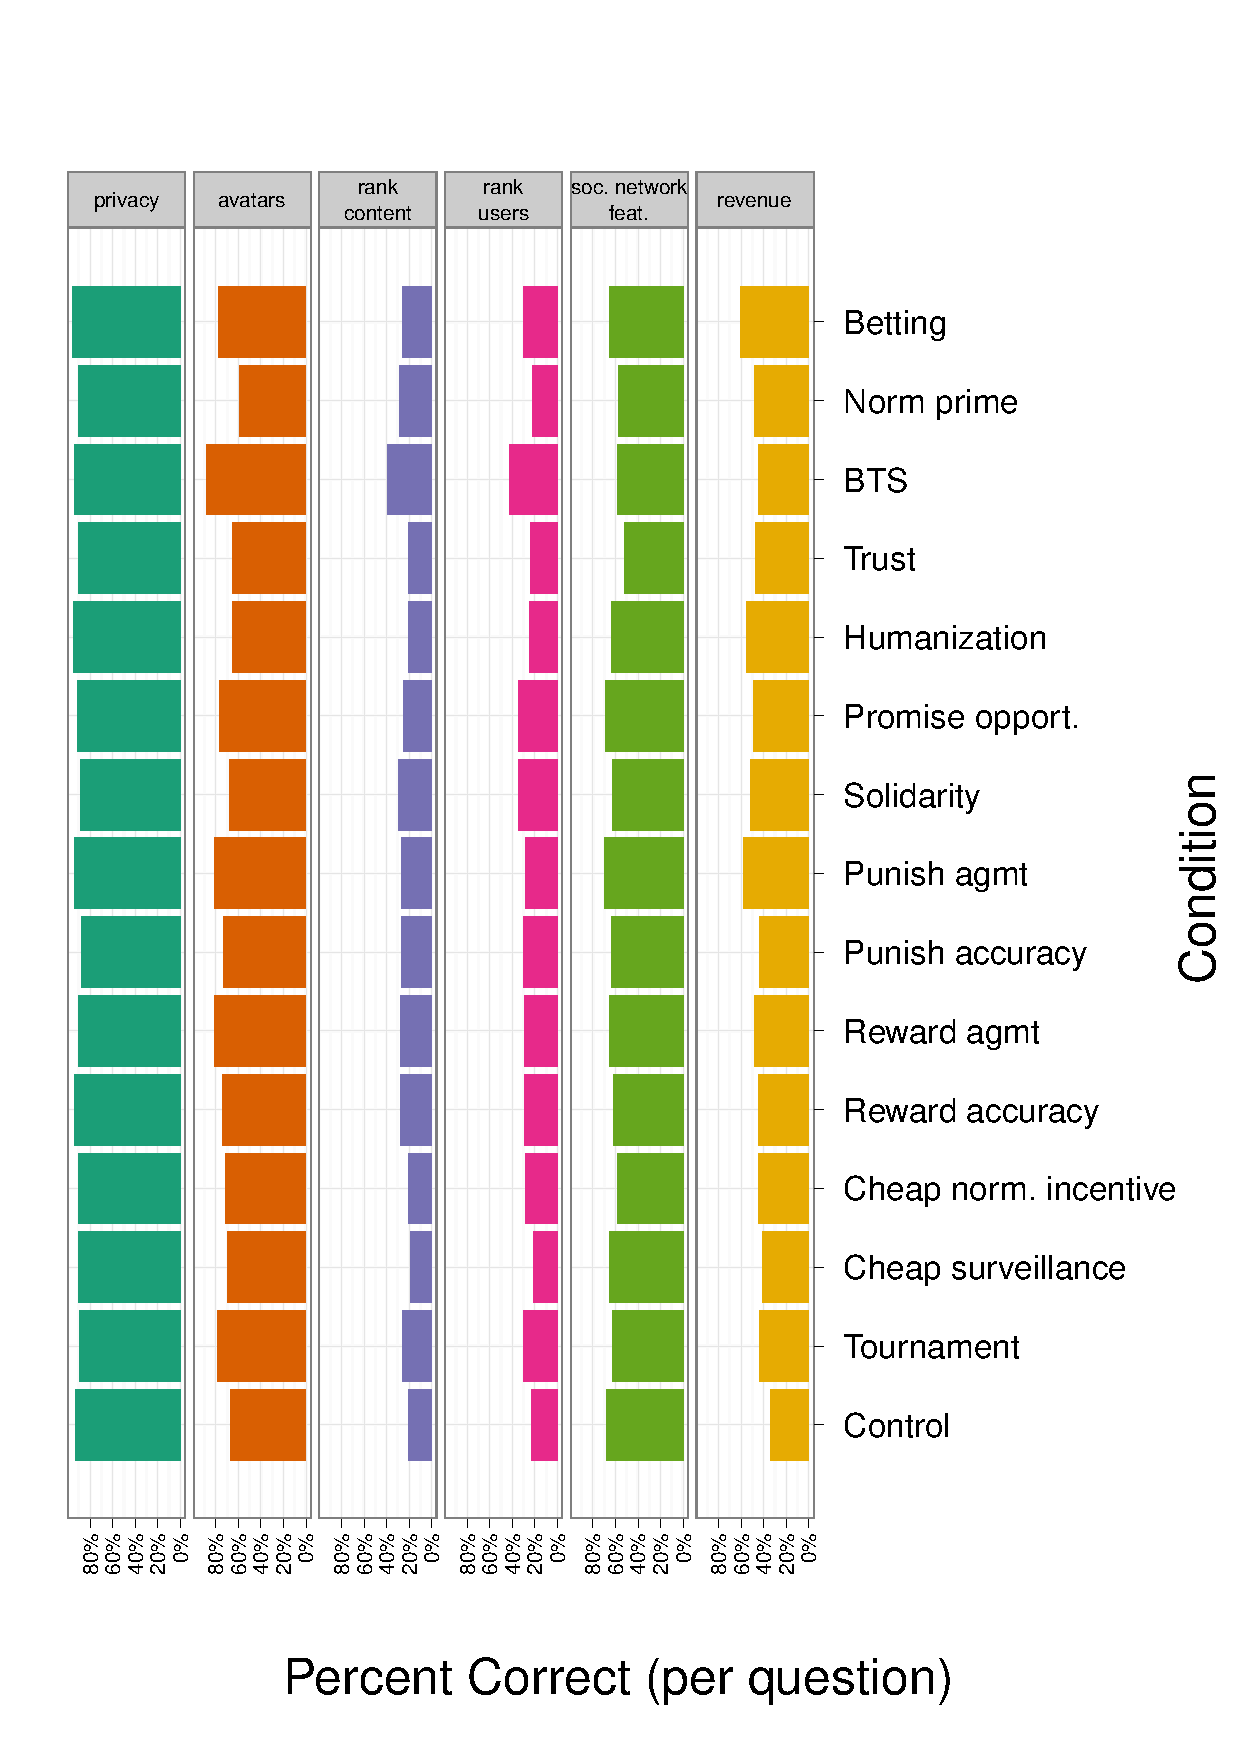
\includegraphics[scale=.35]{../images/per_q}
%\includegraphics[scale=.25]{../images/breakfast_sample_high}
\end{figure} 

\subsection{Aggregate Performance (All Five Questions)}

% aggregated across all conditions 
Figure \ref{fig:AggPerf} illustrates aggregated worker performance
across all five questions and all experimental conditions. On average,
workers did significantly better than chance, which would have yielded
a mean of approximately 1.58 questions correct.  The actual
distribution of responses is strikingly close to normal, with a slight
concentration at 2 and a mean of 2.38.\footnote{This mean reflects
  only the performance of compliers - not the full set of subjects
  exposed to treatment. This corrected (ITT) sample mean was 2.26.}

\begin{figure} 
\centering 
\caption{Worker Performance Distribution - All Conditions \label{fig:AggPerf}}
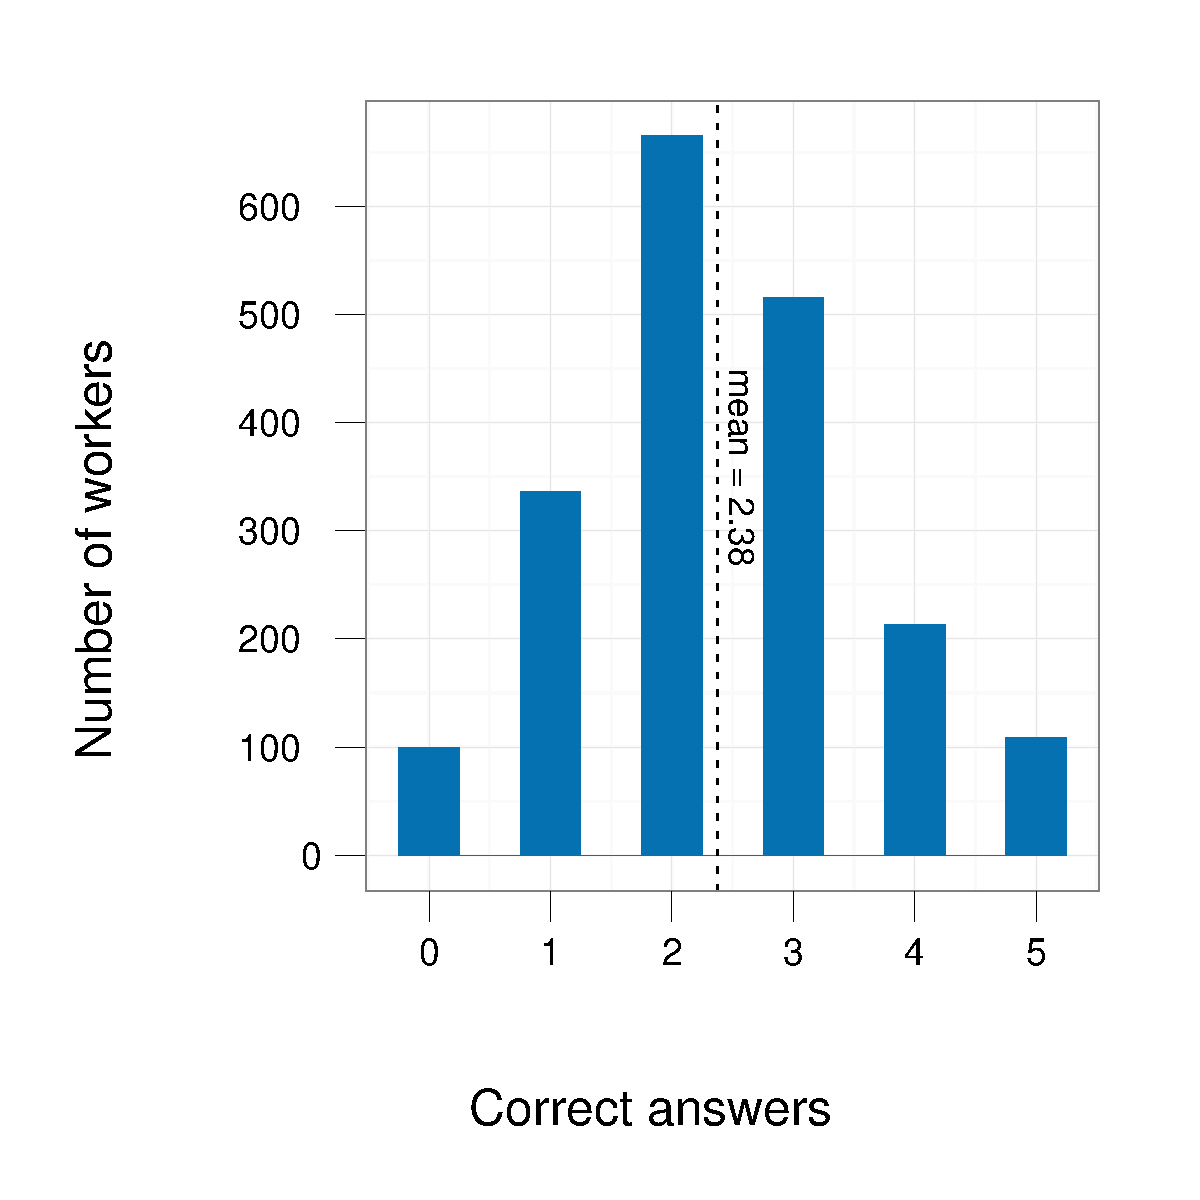
\includegraphics[scale=.25]{../images/AggPerf}
%\includegraphics[scale=.25]{../images/breakfast_sample_high}
\end{figure} 

% compared across conditions 
% ITT estimators & corrected p-values
% TK - insert plot of coefficients and error bars here...
The results of our ITT estimation of average treatment effects (ATE)
are reported in Table \ref{table:agg_results_ITT}.\footnote{The ITT
  estimate of the ATE captures the mean difference in aggregated
  performance between the subjects in each treatment condition and the
  subjects in the control group. The estimates themselves are
  identical with the results of a linear regression on the same
  data. The standard errors are different as are the underlying
  p-values\cite{freedman2008logistic, freedman2008multtreat}. As
  discussed above, all p-values have been corrected using the simple
  Bonferroni correction procedure \cite{shaffer1995, hsu1996}.} To
facilitate the readability of the table, we only report $p \leq 0.05$.

% table 2 - ITT results
\begin{table}[ht]					% set the layout
\begin{center}						% format the layout
\caption{Treatment Effects on Aggregate Performance} % table title
\vspace{8pt}
\begin{threeparttable}
\begin{tabular}{@{}l r r r r@{}}
\toprule
& Mean & ATE\tnote{\dag} & Std. Err. & p-value\tnote{\ddag}\\
\cmidrule(l){2-5}
Control & 2.079 & NA & NA & NA\\
Tournament scoring & 2.310 & 0.232 & 0.142 &\\
Cheap talk-surveillance& 2.027 & -0.052 & 0.131 &\\
Cheap talk-normative& 2.075 & -0.003 & 0.141 &\\
Reward-accuracy& 2.214 & 0.136 & 0.139 &\\
Reward-agreement& 2.421 & 0.342 & 0.135 &\\
Punishment-accuracy& 2.275 & 0.197 & 0.131 & \\
\textbf{Punishment-agreement} & \textbf{2.538} & \textbf{0.459} & \textbf{0.131} & \textbf{0.015}\\
Solidarity& 2.296 & 0.217 & 0.149 &\\
Promise-opportunity& 2.404 & 0.326 & 0.138 &\\
Humanization& 2.171 & 0.092 & 0.142 &\\
Trust& 2.029 & -0.050 & 0.137 &\\
\textbf{Bayesian Truth Serum} & \textbf{2.549} & \textbf{0.471} & \textbf{0.132} & \textbf{0.017}\\
Normative Priming& 2.057 & -0.021 & 0.142 &\\
Betting& 2.438 & 0.359 & 0.137 &\\ 
  \bottomrule
\end{tabular}
  \begin{tablenotes}[para]
  %\begin{flushright}
     \item[\dag]ATE calculated using Intention-to-Treat (ITT) estimators.\\
     \item[\ddag]p-values reported $\leq 0.05$.
 %  \end{flushright}
  \end{tablenotes}
\end{threeparttable}
\label{table:agg_results_ITT}
\end{center}
\end{table}

As described above, we used the ``simple'' Bonferroni correction for
the difference of means comparisons between each treatment group and
the control condition. The results suggest that only two of our
treatments produced a significant improvement in worker performance
over the control: punishment-agreement and Bayesian Truth Serum. In
each case, the effect was approximately .5 above the mean outcome in
control (2.08). Both were significant at $p \leq0.05$.
% In Figure \ref{fig:coef}, we visualize the difference of means comparisons, 
% including error bars.
%\begin{figure} 
%\centering 
%\caption{Here are our results \label{fig:coef}}
%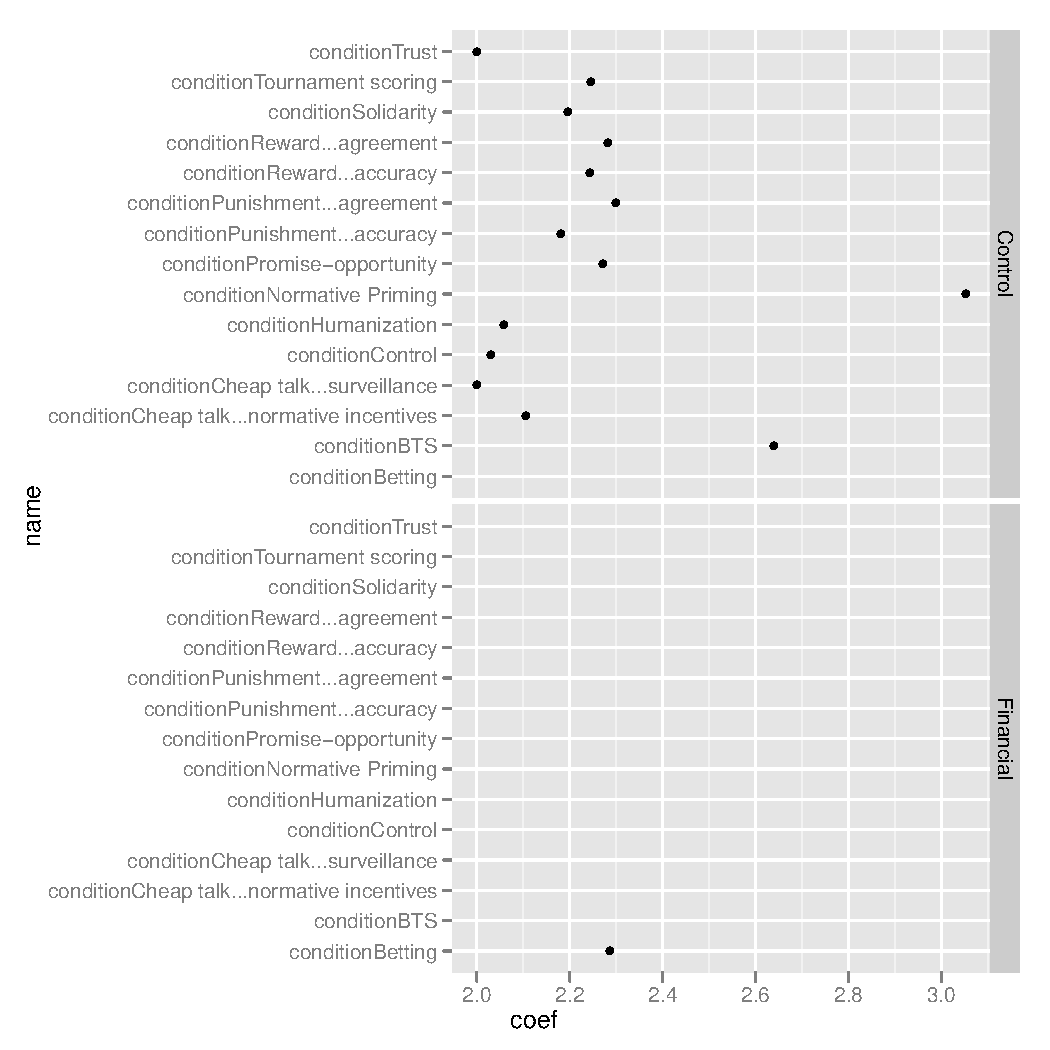
\includegraphics[scale=.5]{../images/coef}
%\includegraphics[scale=.25]{../images/breakfast_sample_high}
%\end{figure} 


\subsection{Post-hoc Demographic Analysis}
To evaluate whether any significant demographic factors may have
affected our estimates, we ran an ordinary least squares (OLS) model
on the outcome variable (aggregate performance score), incorporating
the full set of demographic control variables together with the
treatment assignments. The results of this ``full'' model (not
reported here) suggested that three covariates may have had a
significant association with worker performance despite the
randomization: web-use skills\footnote{To measure this variable, we
  borrowed a survey item from an instrument designed, validated, and
  implemented by Eszter Hargittai in several of her
  studies.\cite{hargittai2009update} The item asks subjects about
  their understanding of two web-browsing tools: ``tabs'' in an
  internet browser and rss feeds. Hargittai found that both items
  correlate highly with independent measures of web-browsing and
  Internet skill.}, household size, and country of residence. To
zero-in on any potentially confounding effects of these variables, we
ran a second model that included only the outcome, the treatment
conditions, and these three covariates.\footnote{The fact that country
  of origin was significant suggested a result consistent with
  previous findings about the differences between workers from India
  and the U.S.\cite{ipeirotis2010}. As a result, we re-coded country
  of residence as a binary variable, indicating whether workers
  self-reported as residing in India or not.}

The second model (reported in Table \ref{table:demog_control_model}) suggests a significant, negative association between performance on our outcome measure, poor web skills and residence in India (both covariates were significant at the $p \leq 0.001$ level after correcting for multiple comparisons). Remarkably, the point estimate of the association between residence in India and the outcome variable dwarfed any of our estimated treatment effects. While household size also remained significant at the $p \leq 0.1$ level, the point estimate dropped below 0.05, implying a weaker association with worker performance.

% table 3 - demog controls
\begin{table}[ht]					% set the layout
\begin{center}						% format the layout
\caption{OLS Regression on Worker Performance} % table title
\vspace{8pt}
\begin{threeparttable}
\begin{tabular}{@{}l r  r r@{}}
\toprule
 & Estimate & Std. Err. & p-value\tnote{\dag}\\
\cmidrule(l){2-4}
(Intercept) & 1.851 & 0.153 & 0.000\\
Tournament scoring & 0.358 & 0.143 &\\
Cheap talk-surveillance & 0.035 & 0.147 &\\
Cheap talk-normative & 0.131 & 0.140 &\\
Reward-accuracy & 0.232 & 0.139 &\\
Reward-agreement & 0.310 & 0.139 &\\
Punishment-accuracy & 0.230 & 0.133 &\\
Punishment-agreement & 0.482 & 0.137 & 0.008\\
Solidarity & 0.291 & 0.144 &\\
Promise-opportunity & 0.398 & 0.139 & 0.074\\
Humanization & 0.136 & 0.141 &\\
Trust & 0.047 & 0.138 &\\
BTS & 0.596 & 0.138 & 0.000\\
Normative Priming & 0.039 & 0.138 &\\
Betting & 0.437 & 0.139 & 0.031\\
Web skill & 0.147 & 0.024 & 0.000\\
Household size  & -0.048 & 0.018 &\\
India resident & -0.739 & 0.068 & 0.000\\
\bottomrule
\end{tabular}
  \begin{tablenotes}[para]
  %\begin{flushright}
	\item Adjusted $R^{2} = 0.127$\\
	\item[\dag]p-values reported $\leq 0.05$.\\
  % \end{flushright}
  \end{tablenotes}
\end{threeparttable}
\label{table:demog_control_model}
\end{center}
\end{table}


\section{Discussion}
%TK-JH: Reasons for effects we did 
%Experimenter effects/
%Might not believe us 
%Existing mturk infrastructure 
%Not salient differences 
%Weird/unusual---might attract attention/Hawthorne effects  

Our results suggest a significant, positive effect of two treatment
conditions - punishment for disagreement with other workers, and
``Bayesian Truth Serum'' - on worker performance in a qualitative
information seeking task on MTurk. None of the ``social'' incentive
schemes altered performance significantly. This suggests that workers
in the MTurk environment may not respond to these sorts of
motivational levers.

Even though we consider examples of financial incentive schemes, the
fact that they alone succeeded where so many other financial incentive
schemes failed hardly implies a ringing endorsement of monetary
incentives by the workers.

Rather, we believe the most compelling explanation of these
treatments' relative success derives from the fact that both asked
workers to prospectively consider how their peers would answer the
information seeking questions. In this regard, it is noteworthy that
the third treatment designed along similar lines (rewards for
agreement with other workers) did not produce significant effects
according to our ITT estimation of difference of means. However, the
rewards-agreement condition did produce one of the larger
point-estimates, suggesting that this sort of prospective reasoning by
workers about their peers may have played an attenuated role in that
group as well.

We also find evidence of a strong association between residence in
India, web skills, and our outcome variable (information seeking task
performance). This implies that culturally-relevant knowledge and
experience online may play an important role mediating workers'
ability to perform the sort of qualitative information seeking task we
asked them to do here.

At the same time, we do not believe that these demographic factors
undermine our findings with regards to the effects of punishment for
disagreement and Bayesian Truth Serum. While the association between
web skills, residence in India, and our outcome variable were quite
strong, their presence in the model hardly altered the point estimates
for the effects of the treatment conditions. This suggests that the
effects we observed for the treatment conditions (at least the
significant ones) were robust and that the randomization worked as a
means for distributing these sub-populations evenly across the
different treatment groups.


\section{Conclusions and Future Work}

The connection we observe between qualitative information seeking performance and treatment conditions asking workers to engage in prospective reasoning about their peers merits further analysis in online and offline settings. In addition, future studies conducted online and with international subject populations should consider the effects of potentially confounding covariates such as country of origin and web-use skills when designing comparable studies. In our case, the randomization proved effective, but this might not be possible in other settings.

Finally, we believe that similar studies should be conducted among other populations online where the existing institutional structure favors other motivational criteria. The rules and norms of the MTurk marketplace strongly favor financial incentives and arms-length relational contracting over more personalistic or socially-oriented modes of exchange. Therefore, it would be interesting to know whether the same incentive schemes would work among a population of Wikipedia contributors who are accustomed to performing similar tasks without any financial payoffs at all.

%Further experimentation is needed. 
%Across different tasks. 
%Populations (Cite Chandler)

\section{Acknowledgments}

The authors thank Yochai Benkler, the Berkman Center for Internet and
Society, and the Law Lab for supporting this work. We are especially
grateful to Jason Callina and Anita Patel for administering the web
application that handled the data collection and storage for this
study. Thanks also to Eszter Hargittai for giving us permission to use
her survey questions. Finally, Dana Chandler as well as five anonymous
reviewers gave us thoughtful feedback on an earlier draft.

John Horton thanks the NSF-IGERT Multidisciplinary Program in
Inequality \& Social Policy for generous financial support (Grant
No. 0333403).

Aaron Shaw thanks Jas Sekhon, Erin Hartman, and Daniel Hidalgo for being really patient. He also thanks Vaughn Hester and John Le of Crowdflower for their feedback on an earlier draft.

Daniel Chen - [insert acknowledgements]

All figures were created with the excellent R package ggplot2, developed by 
Hadley Wickham \cite{wickham2008ggplot2}.
%
\bibliographystyle{abbrv}
\bibliography{turk_raters.bib}

\end{document} 

